%% Преамбула TeX-файла

% 1. Стиль и язык
\documentclass[utf8x, 12pt]{G7-32} % Стиль (по умолчанию будет 14pt)

% Остальные стандартные настройки убраны в preamble.inc.tex.
\sloppy

% Настройки стиля ГОСТ 7-32
% Для начала определяем, хотим мы или нет, чтобы рисунки и таблицы нумеровались в пределах раздела, или нам нужна сквозная нумерация.
\EqInChapter % формулы будут нумероваться в пределах раздела
\TableInChapter % таблицы будут нумероваться в пределах раздела
\PicInChapter % рисунки будут нумероваться в пределах раздела

% Добавляем гипертекстовое оглавление в PDF
\usepackage[
bookmarks=true, colorlinks=true, unicode=true,
urlcolor=black,linkcolor=black, anchorcolor=black,
citecolor=black, menucolor=black, filecolor=black,
]{hyperref}

% Изменение начертания шрифта --- после чего выглядит таймсоподобно.
% apt-get install scalable-cyrfonts-tex

\IfFileExists{cyrtimes.sty}
    {
        \usepackage{cyrtimespatched}
    }
    {
        % А если Times нету, то будет CM...
    }

\usepackage{graphicx}   % Пакет для включения рисунков
\usepackage{pdfpages} 
% С такими оно полями оно работает по-умолчанию:
% \RequirePackage[left=20mm,right=10mm,top=20mm,bottom=20mm,headsep=0pt]{geometry}
% Если вас тошнит от поля в 10мм --- увеличивайте до 20-ти, ну и про переплёт не забывайте:
\geometry{right=20mm}
\geometry{left=30mm}


% Пакет Tikz
\usepackage{tikz}
\usetikzlibrary{arrows,positioning,shadows}

% Произвольная нумерация списков.
\usepackage{enumerate}

% ячейки в несколько строчек
\usepackage{multirow}

% itemize внутри tabular
\usepackage{paralist,array}

% Центрирование подписей к плавающим окружениям
\usepackage[justification=centering]{caption}

% Подсветка кода
%\usepackage{color} %% это для отображения цвета в коде
%\usepackage{listings} %% собственно, это и есть пакет listings


% Настройки листингов.
\ifPDFTeX
% 8 Листинги

\usepackage{listings}

% Значения по умолчанию
\lstset{
  basicstyle= \footnotesize,
  breakatwhitespace=true,% разрыв строк только на whitespacce
  breaklines=true,       % переносить длинные строки
%   captionpos=b,          % подписи снизу -- вроде не надо
  inputencoding=koi8-r,
  numbers=left,          % нумерация слева
  numberstyle=\footnotesize,
  showspaces=false,      % показывать пробелы подчеркиваниями -- идиотизм 70-х годов
  showstringspaces=false,
  showtabs=false,        % и табы тоже
  stepnumber=1,
  tabsize=4,              % кому нужны табы по 8 символов?
  frame=single
}

% Стиль для псевдокода: строчки обычно короткие, поэтому размер шрифта побольше
\lstdefinestyle{pseudocode}{
  basicstyle=\small,
  keywordstyle=\color{black}\bfseries\underbar,
  language=Pseudocode,
  numberstyle=\footnotesize,
  commentstyle=\footnotesize\it
}

% Стиль для обычного кода: маленький шрифт
\lstdefinestyle{realcode}{
  basicstyle=\scriptsize,
  numberstyle=\footnotesize
}

% Стиль для коротких кусков обычного кода: средний шрифт
\lstdefinestyle{simplecode}{
  basicstyle=\footnotesize,
  numberstyle=\footnotesize
}

% Стиль для BNF
\lstdefinestyle{grammar}{
  basicstyle=\footnotesize,
  numberstyle=\footnotesize,
  stringstyle=\bfseries\ttfamily,
  language=BNF
}

% Определим свой язык для написания псевдокодов на основе Python
\lstdefinelanguage[]{Pseudocode}[]{Python}{
  morekeywords={each,empty,wait,do},% ключевые слова добавлять сюда
  morecomment=[s]{\{}{\}},% комменты {а-ля Pascal} смотрятся нагляднее
  literate=% а сюда добавлять операторы, которые хотите отображать как мат. символы
    {->}{\ensuremath{$\rightarrow$}~}2%
    {<-}{\ensuremath{$\leftarrow$}~}2%
    {:=}{\ensuremath{$\leftarrow$}~}2%
    {<--}{\ensuremath{$\Longleftarrow$}~}2%
}[keywords,comments]

% Свой язык для задания грамматик в BNF
\lstdefinelanguage[]{BNF}[]{}{
  morekeywords={},
  morecomment=[s]{@}{@},
  morestring=[b]",%
  literate=%
    {->}{\ensuremath{$\rightarrow$}~}2%
    {*}{\ensuremath{$^*$}~}2%
    {+}{\ensuremath{$^+$}~}2%
    {|}{\ensuremath{$|$}~}2%
}[keywords,comments,strings]

% Подписи к листингам на русском языке.
\renewcommand\lstlistingname{\cyr\CYRL\cyri\cyrs\cyrt\cyri\cyrn\cyrg}
\renewcommand\lstlistlistingname{\cyr\CYRL\cyri\cyrs\cyrt\cyri\cyrn\cyrg\cyri}

\else
\usepackage{local-minted}
\usepackage{mdframed}
\fi

% Полезные макросы листингов.
\include{macros.inc}
\NirOrgLongName{\textsc{НПО <<Рога и Копыта Ltd.}} %% Полное название организации

\NirBoss{Самый Главный}{В.И. Дубин} %% Заказчик, утверждающий НИР

%\renewcommand\otchetcomplement{О НИР} %Можно изменить о чем отчет

%\NirOtchet{\textsc{Отчет о производственной практике}}

%\NirMainBegin{}

\NirManager{Руководитель темы}{А.А. Зипун} %% Название организации

%\NirYear{}%% если нужно поменять год отчёта; если закомментировано, ставится текущий год
\NirTown{г. Санкт-Петербург,} %% город, в котором написан отчёт
% по проекту \No8550: 

% \NirIsAnnotacion{АННОТАЦИОННЫЙ } %% Раскомментируйте, если это аннотационный отчёт

\NirUdk{УДК № 0000}
\NirGosNo{Регистрационный № 123123}

%\NirStage{Этап \No 1}{(заключительный)}{} %%% Этап НИР: {номер этапа}{вид отчёта - промежуточный или заключительный}{название этапа}
%\NirStage{}{}{} %%% Этап НИР: {номер этапа}{вид отчёта - промежуточный или 
\NirFinal{} % Заключительный, если закоментировать то промежуточный
\NirBareSubject{} % Убирает по теме если раскоментить
\NirSubject{Применение сферического коня в вакууме в ООО <<Рога и Копыта Ltd.>>}




\begin{document}

\frontmatter % выключает нумерацию ВСЕГО; здесь начинаются ненумерованные главы: реферат, введение, глоссарий, сокращения и прочее.

\begin{titlepage}

\end{titlepage}

\begin{executors}
\personalSignature{Первый исполнитель}{ФИО}

\personalSignature{Второй исполнитель}{ФИО}
\end{executors}

%\tableofcontents

%\listoffigures

%\listoftables

%\NormRefs % Нормативные ссылки 
% Команды \breakingbeforechapters и \nonbreakingbeforechapters
% управляют разрывом страницы перед главами.
% По-умолчанию страница разрывается.

% \nobreakingbeforechapters
% \breakingbeforechapters

% Также можно использовать \Referat, как в оригинале
\begin{abstract}
Это пример каркаса расчётно-пояснительной записки, желательный к использованию в РПЗ проекта по курсу РСОИ.

Данный опус, как и более новые версии этого документа, можно взять по адресу (\url{https://github.com/rominf/latex-g7-32}).

Текст в документе носит совершенно абстрактный характер.
\end{abstract}

%%% Local Variables: 
%%% mode: latex
%%% TeX-master: "rpz"
%%% End: 


\tableofcontents

%\Defines % Необходимые определения. Вряд ли понадобться
\begin{description}
\item[Распределённый] Слово, которое нельзя употреблять. Но надо протестировать длинные строки в глоссарии.
\item[JCR] Java Content Repository - java API to store data.
\item[OSGI] Open gateway initiative
\item[Replication] Process of copying content from Author instance to Publish instance
\item[Авторский сервер (Author instance)] Сервер, предназначенный для создания контента и управления им. Данный сервер предназначен для работы авторов(контент-менеджеров), которые использую удобный интуитивно понятный интерфейс занимаются наполнением контента сайта. 
\item[Публичный сервер (Publish instance)] Сервер делает контент, создаваемый авторами, доступным для целевой аудитории (пользователей).
\item[Репликация] Механизм в AEM используемый для публикации (копирования) контента с Авторского сервера на Публичный сервер.
\item[Bundle] модули в контексте OSGI спецификации. Представляет из себя jar файл с дополнительной мета информацией.
\end{description}

%%% Local Variables:
%%% mode: latex
%%% TeX-master: "rpz"
%%% End:

\Abbreviations %% Список обозначений и сокращений в тексте
\begin{description}
\item[JCR (Java content repository)] Тип объектной базы данных, используется в системе для хранения, поиска и извлечения иерархических данных.
\item[OSGI] Cпецификация для построения модульных систем для платформы Java \cite{web:osgiSite}.
%\item[Авторский сервер (Author instance)] Сервер, предназначенный для создания контента и управления им. Данный сервер предназначен для работы авторов(контент-менеджеров), которые использую удобный интуитивно понятный интерфейс занимаются наполнением контента сайта.
\item[Экземпляр автора (Author instance)] Среда, предназначенная для создания контента и управления им. Основные пользователи авторы(контент-менеджеры).
\item[Экземпляр публикации (Publish instance)] Среда, предоставляющая пользователям доступ к контенту созданному авторами.
%\item[Публичный сервер (Publish instance)] Сервер делает контент, создаваемый авторами, доступным для целевой аудитории (пользователей).
\item[SSO (Single Sign-On)] Технология единого входа пользователей, благодаря которой владея одной лишь учетной записью пользователь может посещать множество различных ресурсов.
\item[SAML (security assertion markup language)] Язык разметки, основанный на языке XML с помощью которого реализуется SSO. Является открытым стандартом обмена данными аутентификации и авторизации между участниками, в частности, между поставщиком учётных записей и поставщиком услуг.
\item[IdP (identity provider)] Поставщик учетных записей – центральный сервер который хранит аккаунты пользователей.
\item[SP (service provider)] Поставщик услуг – сервис на стороне приложения который обращается к IdP для авторизации пользователя.
\item[Бандл (bundle)] модули в терминах OSGI спецификации. Представляет из себя JAR архив с дополнительной мета информацией.
\item[Лэндскейп (landscape)] Набор элементов аппаратного обеспечения, программного обеспечения и средств, расположенных в определенной конфигурации.
\item[Диспетчер (dispatcher)] Это средство кэширования и / или балансировки нагрузки в Adobe Experience Manager.
\item[Режимы работы (run modes)] Позволяют настраивать экземпляры AEM для конкретных целей и задавать базовую конфигурацию.
\item[AEM Компонент] Настраиваемые компоненты, используемые авторами для наполнения страниц контентом.
\item[Сервис компонент (компонент)] Является основной составляющей декларативных сервисов OSGI спецификации.
%Суть DS в том, что создается дескриптор сервиса: XML-файл, который описывает сервис. Затем данный файл регистрируется в манифесте бандла. Соответственно, OSGi-среда после ресолвинга зависимостей данного бандла автоматически стартует описанные сервисы и переводит бандл в состояние ACTIVE. Естественно, что активатор бандла при этом выполняется.
\end{description}

Определения связанные с архитектурой AEM более подробно рассмотрены в параграфе 3 главы 1.

%%% Local Variables:
%%% mode: latex
%%% TeX-master: "rpz"
%%% End:
 %Абривиатуры вручную, зачем?
%\renewcommand{\nomname}{Список сокращений} % строго перед \printnomenclature
%\printnomenclature % Автоматический список сокращений
%\nomenclature{УОСКВ}{Умственно-отсталый сферический конь в вакууме}

\Introduction

%КОММЕНТ ДО: где, для чего, кем используется система АЕМ. Какие есть проблемы с ней!
Adobe Experience Manager — система управления контентом, осуществляющая хранение, обработку и доставку различных видов контента, предназначенная для крупных компаний, имеющих потребности в управление быстро меняющимся контентом. Созданный контент публикуется на отдельных серверах, оптимизированных для быстрого и надежного чтения хранимых ресурсов. В компаниях использующих систему, может быть развернуто множество AEM сред, где каждая среда будет представлять из себя отдельный проект со своими уникальными модулями и контентом, над которыми ведется активная разработка и внедряются новые модули со своими конфигурациями. Хотя в AEM и имеются механизмы для отслеживания состояния системы, её модулей и компонентов, они проверяют лишь стандартные параметры системы, и не имеют необходимых конфигураций для настройки проверки новых, разработанных модулей и конфигураций.

Целью данной работы является разработка пакета управления мониторингом состояния системы Adobde Experince Manager и интеграция с программой мониторинга Nagios. Для достижения поставленной цели необходимо решить следующие задачи:

\begin{itemize}
\item проанализировать систему Adobe AEM и механизмы мониторинга имеющиеся в системе. Сделать выводы о необходимости разработки данного функционала.
\item Разработать пакет с проверками системы в соответствие с требованиями указанными заказчиком.
\item Реализовать интеграцию проверок с системой Nagios.
\item проверить работоспособность разработанного пакета.
\end{itemize}

В первой главе произведен обзор предметной области, сформулированы требования к разрабатываемому пакету и приведены проектные решения. Вторая глава описывает процесс разработки и тестирования пакета, процессы интеграции с системой Nagios и содержит пользовательскую документацию.

\mainmatter % это включает нумерацию глав и секций в документе ниже

%Исследование
\chapter{Анализ предметной области}
\label{cha:analysis}
%
% % В начале раздела  можно напомнить его цель
%

%\textbf{//КОММЕНТАРИЙ:
%Формулировать задачу обязательно до обзора системы? Если знать архитектуру системы, тогда понятно как такие требования получаются...}

\section{Формулировка задачи}
В данной главе будет рассмотрена система AEM и сформулированы формальные требования на основе первоначальных требований и возможностей системы.

Adobe Experience Manager — система управления контентом, осуществляющая хранение, обработку и доставку различных видов контента в масштабах предприятия. Система предназначена для крупных компаний, имеющих потребности в управление быстро меняющимся контентом, это могут быть как и внутренние корпоративные порталы так и порталы для внешних пользователей. Созданный контент публикуется на отдельных серверах, оптимизированных для быстрого и надежного чтения хранимых ресурсов.

Основные пользователи системы:
\begin{enumerate}
\item Авторы контента или контент-менеджеры - отвечают за наполнения сайтов контентом.
\item Администратор - отвечает за развитие, поддержку работоспособности и безопасности системы.
\item Разработчик - Разработчики работающие с системой занимаются разработкой новых компонентов, шаблонов, и функционала системы.
\item Внешние пользователи - имеют доступ к контенту созданному авторами контента и расположенному на экземплярах публикации.
\end{enumerate}

В компаниях использующих AEM может быть развернуто множество так называемых Лэндскейпов - Наборов элементов аппаратного обеспечения, программного обеспечения и средств, расположенных в определенной конфигурации. Лэндскейпы включают в себя различные наборы серверов в том числе с развернутыми на них AEM средами содержащими экземпляры авторов, публикации и диспетчеры (Приложение A рис.~\ref{fig:complexDeploy}). В крупных компаниях может быть развернуто множество таких сред представляющих из себя самостоятельные порталы или сайты со своим контентом. Такие порталы или сайты могут содержать скрытый контент, доступный только авторизованным внешним пользователям. Как правило, в таких компаниях внешние пользователи имеют один аккаунт для всех систем этой компании т.е применяется технология единого входа рис.~\ref{fig:companyDiagramm}.

\begin{figure}[h]
  \centering
  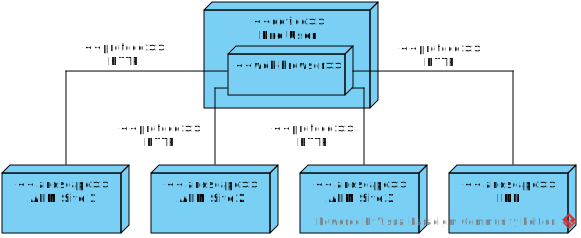
\includegraphics[width=\textwidth]{inc/svg/companyDiagramm}
  \caption{Диаграмма развертывания Лэндскейпов в компании}
  \label{fig:companyDiagramm}
\end{figure}

Несмотря на то что система AEM имеет богатый набор возможностей для авторов контента и администраторов системы, она не имеет встроенных функций для работы с внешними пользователями системы, а именно отсутствует управление авторизацией и контроль доступа для внешних пользователей системы.

Исходя из вышеописанных пунктов возникла необходимость доработки системы с целью реализации взаимодействия с развернутой в компании технологией единого входа и управления авторизацией внешних пользователей на сайтах и порталах компании использующих AEM. Исходные данные и требования полученные от компании: 
\begin{itemize} 
\item В компании развернут поставщик учетных записей, работающий по протоколу SAML.
\item В компании имеется три портала работающих на основе системы AEM.
\item Разрабатываемое решение должно легко внедрятся во все существующие и будущие порталы на базе AEM.
\item Разрабатываемое решение должно поддерживать технологии единого входа рис.~\ref{fig:loginFlow} и выхода рис.~\ref{fig:logoutFlow}.
\item Должна быть возможность использовать различные SAMl привязки, которые должны быть настраиваемыми в каждом приложение.
\item Данные пользователей не должны хранится в хранилище данных системы AEM. Должны хранится только данные сессии, которая имеет короткое время жизни.
\end{itemize}
% Обратите внимание, что включается не ../dia/..., а inc/dia/...
% В Makefile есть соответствующее правило для inc/dia/*.pdf, которое
% берет исходные файлы из ../dia в этом случае.

%\begin{figure}
%  \centering
%  \includegraphics[width=\textwidth]{inc/dia/rpz-idef0}
%  \caption{Рисунок}
%  \label{fig:fig01}
%\end{figure}
%
%В \cite{Pup09} указано, что...
%
%Кстати, про картинки. Во-первых, для фигур следует использовать \texttt{[ht]}. Если и после этого картинки вставляются <<не по ГОСТ>>, т.е. слишком далеко от места ссылки,~--- значит у вас в РПЗ \textbf{слишком мало текста}! Хотя и ужасный параметр \texttt{!ht} у окружения \texttt{figure} тоже никто не отменял, только при его использовании документ получается страшный, как в ворде, поэтому просьба так не делать по возможности.

\begin{figure}[h]
  \centering
  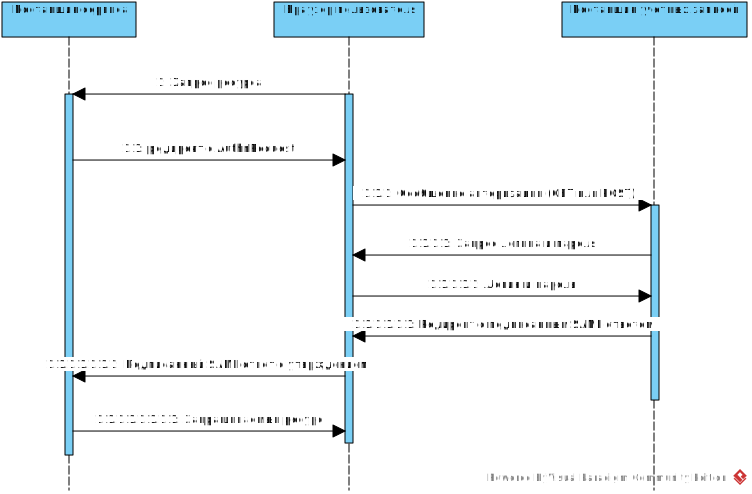
\includegraphics[width=\textwidth]{inc/svg/loginFlow}
  \caption{Диаграмма последовательности, отражающая жизненный цикл технологии единого входа}
  \label{fig:loginFlow}
\end{figure}

\begin{figure}[h]
  \centering
  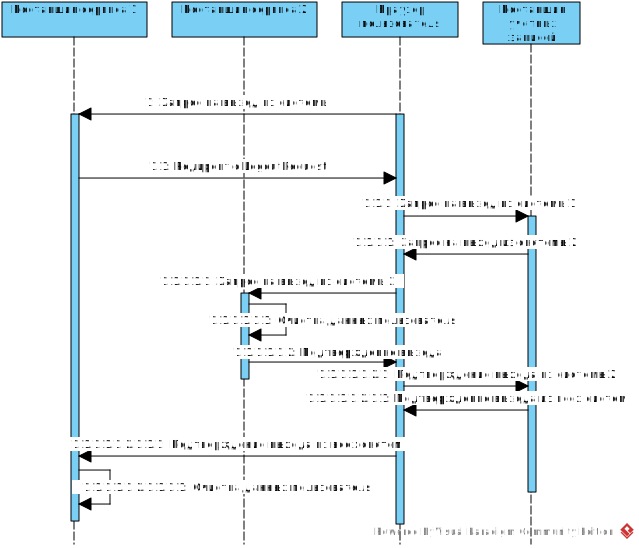
\includegraphics[width=\textwidth]{inc/svg/logoutFlow}
  \caption{Диаграмма последовательности, отражающая жизненный цикл технологии единого выхода}
  \label{fig:logoutFlow}
\end{figure}

\section{Обзор системы и существующих компонентов}

AEM – система построенная с использованием технологии Java. В основе системы лежит фреймворк OSGI. Фреймворк имеет свой контекст, в который и устанавливаются все модули, они взаимодействуют между собой по средствам сервисов зарегистрированных в регистре сервисов рис.~\ref{fig:servicePattern}. Под динамической системой понимается возможность устанавливать, удалять и обновлять модули без перезапуска системы.

\begin{figure}[h]
  \centering
  \includegraphics[width=\textwidth]{inc/svg/servicePattern}
  \caption{Диаграмма архитектуры OSGI}
  \label{fig:servicePattern}
\end{figure}

\subsection{Архитектура AEM}
Основу AEM составляют набор модулей, которые можно условно выделить в 4 компоненты:
\begin{enumerate}
\item Java content repository – один из типов объектной базы данных, созданных для хранения и извлечения иерархических данных. Данные в JCR представляют из собой дерево, состоящее из узлов с ассоциированными с ними свойствами. Эти свойства и являются хранимыми данными, и могут хранить строки, числа или основные примитивные типы данных, а так-же двоичные данные, изображения и.т.д. 
\item Apache Sling – веб-фреймворк построенный по архитектуре REST, отвечающий за доставку контента в контент-ориентированных приложениях с использованием JCR.
\item AEM модули – набор бандлов реализованных компанией Adobe с использованием вышеупомянутых технологий.
\item Пользовательские модули – модули, разрабатываемые разработчиками, и расширяющие функционал системы.
\end{enumerate}

\begin{figure}[h]
  \centering
  \includegraphics[width=\textwidth]{inc/dia/osgi}
  \caption{Архитектура AEM}
  \label{fig:fig02}
\end{figure}

%\textbf{//Комментарий: Если дальше буду говорить про какие-то фишки системы которые проверяю, т.е РЕПЛИКАЦИЯ, Режимы запуска, Жизненный цикл компонентов, то их тоже нужно тут указать?}
%Выделить какой-то абзац под описание ключевых фишек(компонентов) AEM
\subsection{Обзор SAML модулей системы}
В системе имеется SAML модуль - "Adobe Granite - SAML 2.0 Authentication Handler" \cite{web:aemSaml}, предназначенный для интеграции с поставщиком учетных записей. Данный модуль имеет конфигурацию представленную на рис.~\ref{fig:defaultHandlerConfig1} и рис.~\ref{fig:defaultHandlerConfig2}. Рассмотрим подробнее следующие параметры конфигурации:
\begin{itemize}
\item path - путь до контента по которому будет вызван данный обработчик.
\item idpUrl - URL поставщика учетных записей который обрабатывает запросы на авторизацию.
\item idpCertAlias - имя сертификата IdP.
\item serviceProviderEntityId - имя поставщика сервиса сохраненное в IdP.
\item keyStorePassword - пароль от хранилища сертификатов.
\item defaultRedirectUrl - URL на который пользователь будет перенаправлен после успешной авторизации.
\item useEncryption - шифровать сообщения с помощью сертификата из хранилища.
\item createUser - создавать пользователя внутри системы AEM если он не был создан ранее.
\item defaultGroups - группа в которую будет добавлен пользователь при создании.
\item synchronizeAttributes - синхронизировать атрибуты из ответа SAML с атрибутами созданного пользователя.
\item handleLogout - обрабатывать запросы на выход из приложения.
\item logoutUrl - URL выхода, по которому будет вызван данный обработчик.
\end{itemize}

Данный обработчик либо создает пользователя в системе при первой авторизации если выбран параметр "createUser" или требует уже созданного пользователя. Также требуется назначить данных пользователей в соответствующие группы, а также страницам должны быть назначены эти группы. 

Вывод: Несмотря на то что данный подход реализует технологию единого входа он использует хранилище на экземплярах публикации для хранения пользователей, что требует синхронизации между всеми экземплярами публикации и разработки дополнительного функционала для связи атрибутов пользователя с IdP с атрибутами  хранящимся в системе. Необходимость хранить данные пользователей в системе противоречит требованиям и может быть использовано только для экземпляров автора. Также конфигурация реализует только один тип SAML привязки - "HTTP POST binding". Существующий модуль не может удовлетворить поставленные требования, в связи с чем было принято решение разработать новый модуль который будет выступать в роли полноценного поставщика сервиса.

\section{Формальные требования}
Данный раздел уточняет и формирует требования к разрабатываемому модулю.

\subsection{Функциональные требования}
Разрабатываемый модуль должен удовлетворять следующим требованиям:
\begin{itemize}
\item Получает запросы на авторизацию, формирует SAML запрос авторизации и  переправляет пользователя на IdP.
\item Получает запросы на выход из системы формирует SAML запрос выхода из системы и переправляет пользователя на IdP.
\item Получает SAML ответ авторизации, обрабатывает его и при успешном ответе сохраняет cookie пользователя.
\item Получает SAML ответ выхода, обрабатывает его и при успешном ответе удаляет сохраненные cookie пользователя.
\item Получает SAML запрос выхода, обрабатывает его, удаляет сохраненные cookie пользователя и формирует ответ для IdP.
\item Все сообщения должны быть подписаны с использованием сертификата хранящегося в Java Keystore.
\item Должен иметь набор конфигураций.
\end{itemize}

\subsection{Требования к конфигурации}
Модуль должен содержать два вида конфигурации:
\begin{itemize}
\item Base SAML Configuration - содержит единые параметры для всех поставщиков сервиса в системе.
\item Service Provider Configuration - позволяет задать в одной системе несколько поставщиков сервиса со своими параметрами. 
\end{itemize}

Требуемые параметры конфигурации "Base SAML Configuration":
\begin{itemize}
\item Cookie expiration - время жизни cookie в секундах.
\item IdP metadata URI - URL по которому доступны метаданные IdP.
\item JVM Keystore location - путь до Java хранилища ключей.
\item JVM Keystore password - пароль от Java хранилища ключей.
\item SAML Binding type - тип привязки SAML.
\end{itemize}

Требуемые параметры конфигурации "Service Provider Configuration":
\begin{itemize}
\item Service Provider ID - идентификатор поставщика услуг.
\item Service Provider Name - имя поставщика услуг.
\item Certificate Alias - имя сертификата в Java хранилище ключей.
\item Certificate Password - пароль сертификата в Java хранилище ключей.
\item Assertion Consumer Service URI - URL который обрабатывает утверждения полученные от IdP.
\item Cookie Name - имя cookie которые сохраняются при авторизации.
\item Redirect Landing Page URL - URL если необходимо перенаправление пользователя после авторизации.
\item Error Redirect URL - URL если обрабатывающий ошибку произошедшую в процессе авторизации.
\end{itemize}

\section{Заключение}
В данной главе был произведен обзор системы и рассмотрены сценарии при которых возникает необходимость разработки нового модуля для управления авторизацией в системе AEM с использованием SAML. Встроенные механизмы для реализации авторизации с помощью SAML не соответствуют всем требованиям заказчика. Было принято решение разработать новый модуль который можно будет использовать во всех проектах заказчика использующих AEM.


%%% Local Variables:
%%% mode: latex
%%% TeX-master: "rpz"
%%% End:

%Постановка задачи и проектирование
\chapter{Проектирование}
\label{cha:design}

%В данном разделе реализуется новая всячина.
При разработки нового модуля было решено использовать существующие фреймворки, реализующие стандарт SAML. В данной главе приведен обзор выбранных фреймворков и произведен анализ возможности их интеграции с системой AEM. На основе выбранного фреймворка спроектирована архитектура разрабатываемого модуля. 

\section{Выбор фреймворка}
Список фреймворков, рассматриваемых при разработке, был получен с официального сайта SAML \cite{web:samlFrameworksOasis} и со страницы в википедии \cite{web:samlFrameworksWiki}. Поскольку AEM основана на Java были выбраны только совместимые с системой фреймворки. 

\subsection{Обзор выбранных фреймворков}
Для сравнения выбранных фреймворков была составлена таблица 2.1, в которой выполняется сравнение по следующим параметрам:

\begin{itemize}
\item Поддержка - осуществляется ли поддержка библиотеки, когда выпущена последняя версия.
\item Количество запросов на stackoverflow - количество запросов на stackoverflow показывает насколько популярна библиотека.
\item Примеры и документация - наличие примеров и документации.
\end{itemize}

\begin{longtable}{|p{3cm}|p{47mm}|p{30mm}|p{35mm}|}
  \caption{Сравнение SAML фреймворков}
  \label{tab:tabular}
  \\ \hline
  Название & Поддержка & Количество запросов на stackoverflow & Примеры и документация \\
  \hline \endfirsthead
  \subcaption{Продолжение таблицы~\ref{tab:tabular}}
  \\ \hline \endhead
  \hline \subcaption{Продолжение на след. стр.}
  \endfoot
  \hline \endlastfoot
  Название      
  & Поддержка 
  & Количество запросов на stackoverflow 
  & Примеры и документация \\
  \hline
  OpenSAML 3  
  & Поддерживается, последняя версия: март 2017
  & 399
  & Есть примеры, книги, плохая документация на официальном сайте \\
  \hline
  OneLogin       			   
  & Поддерживается, последняя версия: ноябрь 2018
  & 324
  & Есть примеры, хорошая документация на официальном сайте \\
  \hline
  Spring Security SAML                
  & Поддерживается, последняя версия: март 2019
  & боле 500
  & Есть примеры, плохая документация на официальном сайте \\
  \hline
  Pac4j       			   
  & Поддерживается, последняя версия: февраль 2019
  & 16
  & Есть примеры, хорошая документация на официальном сайте \\
  \hline
\end{longtable}	

Составленная таблица не позволяет однозначно сказать какое решение подойдет лучше всего, поэтому с использованием каждого фреймворка был разработан прототип приложения, формирующий сообщение авторизации с заданным параметрами-заглушками, пример сообщения приведен в листинге \ref{lst:authnRequestExample}. Разработанные прототипы позволят сравнить возможности настройки фреймворков, удобство использования и доработок под свои нужны.

\begin{longlisting}
\inputminted[linenos,frame=single]{xml}{inc/src/authnRequestExample}
\caption{Пример SAML AuthnRequest} 
\label{lst:authnRequestExample}
\end{longlisting}

\subsection{Интеграция фреймворков с AEM}
При попытке интеграции разработанных прототипов со средой AEM все прототипы оказались не работоспособны. В результате анализа было выявлено что это частое явление при использование сторонних библиотек не оптимизированных для работы в среде OSGI \cite{web:usingClassLoaders}.

Данная проблема возникает из-за различий в загрузки классов классического Java приложения и среды OSGI. В классическом Java приложении существует один загрузчик классов на все приложение, в среде OSGI для каждого модуля существует свой загрузчик классов. Все фреймворки используют для загрузки классов контекст который не знает о существование среды OSGI, листинг \ref{lst:threadContext}, и поэтому происходит ошибка при загрузки файлов. Для решения данной проблемы необходимо переопределить код фреймворка, который отвечает за загрузку классов.

\begin{listing}[H]
\inputminted[linenos,frame=single]{java}{inc/src/threadContext}
\caption{Загрузчик классов не работающий в среде OSGI} 
\label{lst:threadContext}
\end{listing}

\subsection{Заключение}
Составленная таблица и разработанный прототип позволили подробно изучить фреймворки и выделить плюсы и минусы их использования при разработки. Ниже приведены выводы по каждому фреймворку:

\begin{itemize}
\item OpenSAML 3 - Наиболее соответствующая стандарту реализация. Низкоуровневый фреймворк который отвечает только за формирование XML сообщений. Активно развивается и поддерживается. Требуется переопределение стартовой конфигурации так как не предназначен для работы в OSGI среде, однако из-за своей низкоуровневой архитектуры и модульности это не составляет труда. Имеет плохую официальную  документацию но множество примеров использования, так-же имеется печатное руководство по использованию \cite{web:openSamlBlog}.
\item OneLogin - Не предназначен для работы в OSGI среде, сложно изменить инициализацию. Работает с ограниченным набором провайдеров авторизации. Имеются подробные примеры использования на официальном сайте а также на stackoverflow.
\item Spring Security SAML - Использует внутри OpenSAML 2, выполняет оборачивание базовых методов, но не поддерживает все типы сообщений доступные в стандарте. Используется устаревшая версия OpenSAML 2. Плохо совместим с OSGI средой. Поддерживает большинство популярный провайдеров идентификации. Имеет большое количество примеров использования.
\item Pac4j- Использует внутри OpenSAML3, оборачивает базовые методы что позволяет реализовывать функции гораздо быстрее. Ограничен в доступных методах и настройках. Не предназначен для работы в OSGI среде. В отличие от OpenSAML 3 инициализация не может быть легко изменена что делает библиотеку не удобной в использование и требует большего времени доработки.
\end{itemize}

В результате анализа было принято решение разрабатывать модуль с применением фреймворка – OpenSAML 3. Несмотря на то что другие фреймворки предоставляют больше готовых решений они не реализуют все возможности стандарта и имеют трудности при интеграции со средой AEM.

\section{Проектные решения}
На основе требований и выбранного фреймворка можно спроектировать структуру разрабатываемого модуля. Поскольку Open SAML 3 является низкоуровневым фреймворком и в основном необходим для генерации XML сообщений было принято решение выделить следующую структуру пакетов модуля:

\begin{enumerate}
\item authentication - принимает запросы на аутентификацию и ответы от провайдера авторизации, обрабатывает и определяет их тип. Отправляет запросы к провайдеру авторизации вместе с составленными сообщениями. Сохраняет сессию пользователя в куки. Пакет имеет следующую структуру рис.~\ref{fig:coreAuthn}:
\begin{enumerate}
\item security.ecryption - пакет содержащий функции шифрования и дешифрования строк.
\item servlets - пакет содержащий сервлеты обрабатывающие запросы а также обработчики сообщений.
\item utils - пакет утилит.
\item models - пакет моделей пользователя и куки.
\end{enumerate}
\item saml - генерирует SAML сообщения с использованием выбранного фреймворка, выполняет валидацию принятых сообщений, а также выполняет настройку библиотеки при установке в систему. Имеет пакет конфигурации, который позволяет использовать проектируемый модуль во всех системах AEM с различными настройками поставщика сервиса. Пакет имеет следующую структуру рис.~\ref{fig:coreSaml}:
\begin{enumerate}
\item bundle - выполняет конфигурацию модуля при его установки в OSGI среду.
\item validator - содержит классы выполняющие валидацию утверждений полученных от IdP.
\item messages - содержит классы работы с сообщениями авторизации.
\item configuration - содержит конфигурации модуля.
\item security - содержит классы извлекающие сертификаты из Java хранилища ключей и осуществляющие подпись всех XML сообщений.
\item utils - пакет утилит, необходимый для первоначальной настройки Open SAML 3 фреймворка.
\end{enumerate}
\item ids.configuration - вспомогательный пакет, не относящийся к работе напрямую но созданный в связи с дополнительными требованиями полученными в процессе разработки. Содержит конфигурацию которая задает параметры IdP и JavaScript который позволяет пользователю проходит авторизацию на стороне сайта или портала без перехода на сайт IdP.
\end{enumerate}		

\begin{figure}[h]
  \centering
  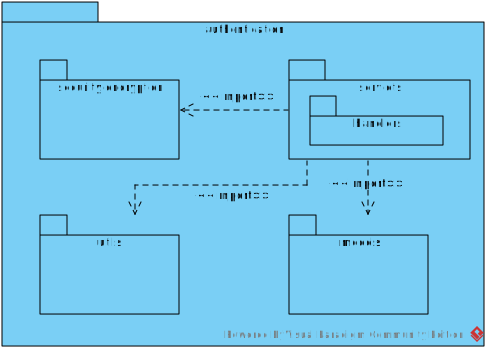
\includegraphics[width=\textwidth]{inc/svg/coreAuthn}
  \caption{Диаграмма структуры пакета authentication}
  \label{fig:coreAuthn}
\end{figure}

\begin{figure}[H]
  \centering
  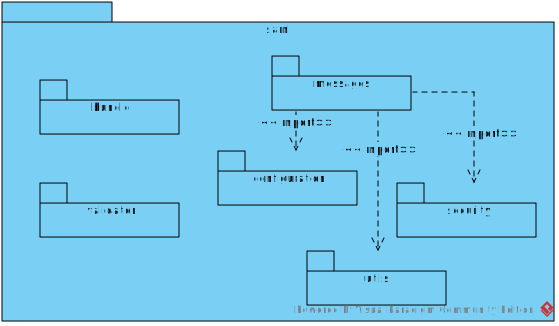
\includegraphics[width=\textwidth]{inc/svg/coreSaml}
  \caption{Диаграмма структуры пакета saml}
  \label{fig:coreSaml}
\end{figure}

\section{Заключение}
В данной главе был выбран фреймворк реализующий стандарт SAML с использованием которого будет разработан модуль. На основе выбранного фреймворка была спроектирована архитектура разрабатываемого модуля.

%%% Local Variables:
%%% mode: latex
%%% TeX-master: "rpz"
%%% End:

%Реализация
\chapter{Реализация}
\label{cha:impl}

\section{Разработка}
Разработку модуля необходимо начать с интеграции фреймворка Open SAML 3 с OSGI средой, затем будет рассмотрена разработка модулей авторизации и работы с SAML сообщениями.

\subsection{Интеграция Open SAML 3 со средой OSGI}
Как было выявлено в процессе выбора фреймворка, Open SAML 3 выполняет первоначальную инициализацию, загружая необходимые ресурсы и классы используя загрузчик классов не знающий о существование среды OSGI. Стандартный процесс инициализации фреймворка предполагает вызов метода initialize() сервиса org.opensaml.core.config.InitializationService. Данный сервис загружает все объекты которые необходимы для работы и регистрирует их в Java среде использую Java Services API с помощью сервиса org.opensaml.core.config.ConfigurationService. Для использования фреймворка в OSGI среде необходимо переопределить инициализацию фреймворка и поведение вышеописанных сервисов.

Для решения данной задачи было разработано три класса выполняющие первоначальную инициализацию фреймворка:
\begin{enumerate}
\item Activator - класс в котором заданы действия выполняющиеся при запуске модуля. В данном приложение метод активации извлекает загрузчик классов этого модуля и передает его в класс инициализации Open SAML 3, после чего вызывается метод SamlInitializationSupport.initialize(), листинг \ref{lst:activator}.
\item InitializationXMLConfigurator - класс наследует XMLConfigurator и подменяет загрузчик классов в методе createClassInstance(), листинг \ref{lst:xmlConfigurator}.
\item SamlInitializationSupport - основной класс инициализации, хранит все конфигурации и загрузчик классов модуля, приложение А листинг \ref{lst:samlInitialization}. Содержит следующие ключевые методы:
\begin{enumerate}
\item initializeXMLTooling - инициализирует все XML сервисы, перечисленные в списке конфигураций: configs[], использует переопределённый InitializationXMLConfigurator.
\item initializeAlgorithmRegistry -инициализирует алгоритмы используя загрузчик классов модуля.
\item initializeParserPool - инициализирует XML парсер.
\end{enumerate}
\end{enumerate}

\begin{longlisting}
\inputminted[linenos,frame=single]{java}{inc/src/Activator}
\caption{Метод активации модуля} 
\label{lst:activator}
\end{longlisting}

\begin{longlisting}
\inputminted[linenos,frame=single]{java}{inc/src/InitializationXMLConfigurator}
\caption{Класс инициализации XML конфигураций} 
\label{lst:xmlConfigurator}
\end{longlisting}

Данные классы выполняют инициализацию фреймворка Open SAML 3 во время активации модуля. Дальнейшая работа с фреймворком не требует специальных настроек и может выполняться как в классическом Java приложение.

\subsection{Подмодуль authentication}
Данный пакет предназначен для обработки запросов поступающих к сервису и является входной точкой приложения, диаграмма классов пакета представлена в приложение А рис.~\ref{fig:authenticationModule}. Пакет содержит следующие подпакеты и классы:
\begin{enumerate}
\item security.encryption
\item servlets
\item utils
\item Constatns
\item User
\item UserCookie
\end{enumerate}

\paragraph{Пакет security.encryption} содержит классы DesEncryptor и DesDecryptor  выполняющие шифрование и дешифрование значения куки с использованием алгоритма RSA/ECB/PKCS1Padding и стандартного Java класса javax.crypto.Cipher листинг \ref{lst:cipher}. Классы имеют методы decrypt() и encrypt() принимающие в качестве параметров строку которую необходимо зашифровать и ID поставщика сервиса. Ключ для шифрования извлекается из Java хранилища ключей, имя ключа извлекается из конфигурации модуля относящейся к переданному поставщику сервиса.

\begin{listing}[H]
\inputminted[linenos,frame=single]{java}{inc/src/cipher}
\caption{Код получения шифра} 
\label{lst:cipher}
\end{listing}

\paragraph{Пакет servlets} содержит сервлеты которые обрабатывают пользовательские запросы:
\begin{enumerate}
\item LoginServlet - Данный сервлет обрабатывает запросы на авторизацию либо ответы от поставщика учетных записей и имеет два сценария срабатывания:
\begin{enumerate}
\item Если поступил запрос на авторизацию от пользователя, то извлекается ID поставщика сервиса из селектора запроса с помощью которого будет получена конфигурация данного поставщика, затем составляется сообщение для поставщика учетных записей и выполняется его отправка.
\item Если в параметрах запроса обнаружен SAML ответ на авторизацию, то будет вызван обработчик AuthenticationResponseHandler.
\end{enumerate}
\item LogoutServlet -  Данный сервлет обрабатывает запросы на выход из системы либо ответы от поставщика учетных записей и имеет три сценария срабатывания:
\begin{enumerate}
\item Если в параметрах запроса обнаружен SAML ответ на запрос выхода из системы, то будет вызван обработчик LogoutResponseHandler. 
\item Если в параметрах запроса обнаружен SAML запрос на выход из системы, что означает запрос на выход из системы со стороны поставщика учетных записей, то будет вызван обработчик LogoutRequestHandler. 
\item Если поступил запрос на выход из системы от пользователя, получается конфигурация поставщика сервиса по аналогии с запросом авторизации, затем составляется и отправляется сообщение для поставщика учетных записей.
\end{enumerate}
\item UserInfo - Сервлет используемый для тестирования и влидации. Отображает информацию которая хранится о пользователи в куки.
\end{enumerate}

Данный пакет также содержит следующие обработчики запросов:
\begin{enumerate}
\item AuthenticationResponseHandler - обрабатывает и валидирует SAML ответы от поставщика учетных записей с помощью класса SamlAuthnResponseValidator. Если ответ прошел валидацию создается пользователь из полученных параметров SAML Assertion и сохраняются куки пользователя, пользователь перенаправляется на страницу для авторизованных пользователей либо на запрашиваемый ресурс.
\item LogoutRequestHandler - обрабатывает SAML запрос на выход из системы полученный от поставщика учетных записей. Удаляет куки пользователя, формирует и отправляет SAML сообщение для поставщика учетных записей о выполненной операции, после чего переправляет пользователя на страницу для не авторизованных пользователей.
\item LogoutResponseHandler - обрабатывает SAML ответ подтверждающий выход из системы полученный от поставщика учетных записей. Удаляет куки пользователя и переправляет его на страницу для не авторизованных пользователей.
\end{enumerate}

\paragraph{Пакет utils} содержит класс AuthUtils предназначенный для проверки передаваемых параметров на наличие XSS уязвимостей.

\paragraph{Класс Constatns} содержит константы путей по которым доступны сервлеты и значение куки которое должно быть задано при выходе из системы.
\paragraph{Класс User} представляет из себя модель пользователя и содержит все поля которые могут быть переданы поставщиком учетных записей вместе с ответом авторизации.
\paragraph{Класс UserCookie} представляет из себя модель куки пользователя и содержит набор значений которые хранятся в куки для пользователя:
\begin{enumerate}
\item userName - ID авторизованного пользователя.
\item sessionIndex - индекс сессии полученный от поставщика учетных записей.
\item user - объект пользователя полученный от поставщика учетных записей.
\end{enumerate}

\subsection{Подмодуль saml} 
Данный пакет предназначен для работы с SAML сообщениями а также конфигурации модуля, диаграмма классов пакета представлена в приложение А рис.~\ref{fig:samlModule}. Пакет содержит следующие подпакеты и классы:
\begin{enumerate}
\item bundle
\item configuration
\item messages
\item security
\item utils
\item validator
\end{enumerate}

\paragraph{Пакет bundle} содержит единственный класс Activator который был подробно рассмотрен в разделе "Интеграция Open SAML 3 со средой OSGI".
\paragraph{Пакет configuration} содержит сервисы конфигурации которые будут рассмотрены подробно в следующей секции данной главы.
\paragraph{Пакет messages} содержит классы осуществляющие генерацию SAML сообщений которые отправляются поставщику учетных записей и состоит из следующих классов:
\begin{enumerate}
\item BindingType - перечисляемый тип который содержит виды SAML привязки доступные в приложение. В текущей версии поддерживаются только POST и REDIRECT.
\item AbstractSamlMessage - абстрактный класс который содержит общие методы для всех SAML сообщений. Содержит следующие методы для работы с сообщениями:
\begin{enumerate}
\item generateUUID - генерирует ID которое служит идентификатором сообщения.
\item generateSigningParameters - генерирует параметры необходимые для подписи сообщения.
\item appendSigningData - подписывает сообщение в соответствие с типом привязки.
\item signObject - подписывает сообщение с помощью сертификата для типа привязки POST.
\item sendMessageToIDP - собирает сообщение и отправляет его поставщику учетных записей.
\end{enumerate}
\item SAML2AuthnRequestMessage - сообщение авторизации, код генерации сообщения в приложении А листинг \ref{lst:authMessage}.
\item SAML2LogoutRequestMessage - сообщение выхода из системы, код генерации сообщения в приложении А листинг \ref{lst:logoutMessage}.
\item SAML2LogoutResponseMessage - сообщение ответ на запрос выхода из системы со стороны поставщика учетных записей, код генерации сообщения в приложении А листинг \ref{lst:logoutResponseMessage}.
\end{enumerate}
\paragraph{Пакет security} содержит класс X509 который осуществляет взаимодействие с Java хранилищем ключей и предоставляет ключи для подписи сообщений или валидации полученных сообщений.
\paragraph{Пакет utils} содержит классы инициализации которые были рассмотрены ранее, а также вспомогательный класс SamlUtils со следующими методами:
\begin{enumerate}
\item getMessage - используется в обработчиках для извлечения SAML сообщения из запроса.
\item getMessageEncoder - используется в SAML сообщениях для задания сообщению кодировщика в соответствие с указанным в конфигурации типом  привязки.
\end{enumerate}
\paragraph{Пакет validator} содержит единственный класс SamlAuthnResponseValidator, который выполняет валидацию SAML ответа от поставщика учетных записей на запрос авторизации. Код валидации представлен в приложении А  листинг \ref{lst:validation}. В процессе валидации проверяется что структура сигнатуры верна и она подписана сертификатом который принадлежит поставщику учетных записей. Валидатор сигнатуры использует для работы Java Service API и требует отдельного переопределения для использования загрузчика классов модуля, листинг \ref{lst:activator}.

\begin{longlisting}
\inputminted[linenos,frame=single]{java}{inc/src/validatorLoader}
\caption{Код переопределения загрузчика классов валидатора} 
\label{lst:validatorLoader}
\end{longlisting}

\subsection{Конфигурация модуля}
Конфигурация модуля находится в пакете saml и содержит два вида конфигурации:
\begin{enumerate}
\item SamlConfigurationImpl - конфигурация которая содержит все элементы задающие используемый в системе поставщик учетных записей. Имеет следующие параметры:
\begin{enumerate}
\item idp.metadata.uri - URL метаданных IdP из которых извлекаются URL авторизации и выхода из системы.
\item jvm.keystore.location - путь до Java хранилища ключей в системе.
\item jvm.keystore.password - пароль Java хранилища ключей.
\item sp.saml.binding.type - тип SAML привязки, выбираемый параметр который может быть POST или REDIRECT.
\item ids.cookie.expiry - время жизни куки пользователя, если -1 время жизни приравнивается к времени жизни сессии.
\end{enumerate}
\item SamlServiceProviderConfigurationFactory - конфигурация которая задает параметры поставщика сервиса в системе. В системе может использоваться несколько различных поставщиков учетных записей с различными конфигурациями. Имеет следующие параметры:
\begin{enumerate}
\item sp.acs.uri - URL для обработки ответов от IdP и обработки утверждений.
\item sp.name - имя поставщика сервиса.
\item sp.id - идентификатор поставщика сервиса, используется для доступа к данной конфигурации.
\item x509.certificate.alias - имя сертификата который используется для подписи сообщений и валидации ответов от IdP.
\item x509.certificate.password - пароль от сертификата.
\item wcms.ids.cookie.name - имя под которым сохраняются куки пользователя.
\item wcms.ids.redirect.landingPage.url - URL на который переправляется пользователь после успешной авторизации.
\item wcms.ids.error.redirect.url - URL ошибок на который переправляется пользователь при возникновение ошибок в процессе авторизации.
\item wcms.ids.redirect.pattern - проверяет что URL перенаправления валдиный. 
\item cookie.additional.attributes - дополнительные параметры полученные от IdP.
\end{enumerate}
\item IdsConfigurationImpl - вспомогательная конфигурация, которая задает параметры позволяющие пользователю проходить авторизацию на стороне сайта или портала без перехода на сайт IdP. Имеет следующие параметры:
\begin{enumerate}
\item ids.host.name - адрес сервиса.
\item ids.port.number - порт сервиса.
\item ids.logon.ui.script - путь до скрипта пользовательского интерфейса.
\item ids.user.profile.script - путь до скрипта модального окна IdP.
\end{enumerate}
\end{enumerate}

\section{Тестирование}

Для оценки соответствия приложения заявленным требованиям было выполнено функциональное тестирование по тестовым сценариям. Тестирование проходило в два этапа, локально и на тестовом сервере компании. В тестирование принимало участие три независимых проекта использующих данный модуль и единый для всех поставщик учетных записей. Для проверки сценариев использовались бразуерные SAML плагины которые отображали SAML сообщения в запросах:

\begin{itemize}
\item SAML DevTools extension - для Chrome.
\item SAML-tracer - для Fire Fox.
\end{itemize}

\subsection{Тестирование сценария авторизации}
В таблице \ref{tab:testAuthn} приведены результаты тестирование сценария авторизации при котором использовалось два ресурса на которых выполнялся вход с настроенной конфигурацией используемого в компании поставщика учетных записей. Для обоих ресурсов использовался один и тот-же аккаунт.

\begin{longtable}{|p{5cm}|p{5cm}|l|}
  \caption{Результаты тестирования сценария авторизации}
  \label{tab:testAuthn}
  \\ \hline
  Шаг сценария & Ожидаемый результат & полученный результат  \\
  \hline \endfirsthead
  \subcaption{Продолжение таблицы~\ref{tab:testAuthn}}
  \\ \hline \endhead
  \hline \subcaption{Продолжение на след. стр.}
  \endfoot
  \hline \endlastfoot
  Пользователь отправляет запрос авторизации  
  & Приложение генерирует сообщение и перенаправляет пользователя на IdP вместе с этим сообщением
  & Соответствует \\
  \hline
  Пользователь проходит авторизацию на стороне IdP       			   
  & IdP перенаправляет пользователя обратно на сторону приложение вместе с SAML утверждением которое содержит данные пользователя и данные о созданной сессии
  & Соответствует \\
  \hline
  Приложение обрабатывает ответ               
  & Данные пользователя о сессии сохранены в куки и пользователю доступен контент
  & Соответствует \\
  \hline
\end{longtable}	

\subsection{Тестирование сценария выхода}
Для тестирования сценариев выхода из системы было использовано два портала использующих разработанный модуль.
\begin{itemize}
\item пользователь успешно авторизован на одном портале после чего инициализирует процесс выхода из системы (таблица \ref{tab:singleLogout}). 
\item пользователь авторизован на двух порталах и инициализирует процесс выхода из системы на одном из них (таблица \ref{tab:tripleLogout}).
\end{itemize}

\begin{longtable}{|p{5cm}|p{5cm}|l|}
  \caption{Результаты тестирования сценария выхода из системы для одного портала}
  \label{tab:singleLogout}
  \\ \hline
  Шаг сценария & Ожидаемый результат & полученный результат  \\
  \hline \endfirsthead
  \subcaption{Продолжение таблицы~\ref{tab:singleLogout}}
  \\ \hline \endhead
  \hline \subcaption{Продолжение на след. стр.}
  \endfoot
  \hline \endlastfoot
  Пользователь отправляет запрос выхода из системы  
  & Приложение генерирует сообщение и перенаправляет пользователя на IdP вместе с этим сообщением 
  & Соответствует \\
  \hline
  IdP удаляет сессию пользователя на своей стороне и посылает приложению сообщение об успешном выходе из системы       			   
  & Приложение получает ответ об успешном выходе из системы и очищает куки пользователя, после чего перенаправляет его на страницу авторизации
  & Соответствует \\
  \hline
\end{longtable}	

\begin{longtable}{|p{5cm}|p{5cm}|l|}
  \caption{Результаты тестирования сценария выхода из системы для нескольких порталов}
  \label{tab:tripleLogout}
  \\ \hline
  Шаг сценария & Ожидаемый результат & полученный результат  \\
  \hline \endfirsthead
  \subcaption{Продолжение таблицы~\ref{tab:tripleLogout}}
  \\ \hline \endhead
  \hline \subcaption{Продолжение на след. стр.}
  \endfoot
  \hline \endlastfoot
  Пользователь отправляет запрос выхода из системы  
  & Приложение генерирует сообщение и перенаправляет пользователя на IdP вместе с этим сообщением 
  & Соответствует \\
  \hline
  IdP находит все сессии, генерирует сообщения выхода для всех сервисов по очереди и перенаправляет пользователя на эти сервисы один за одним для осуществления выхода из системы.
  & Приложение получает запрос на выход из системы от IdP, очищает куки пользователя, генерирует ответ информирующий IdP об успешном выходе из системы и перенаправляет пользователя на IdP
  & Соответствует \\
  \hline
  IdP получает ответ о выходе из системы последнего сервиса, он генерирует сообщение ответ для приложения инициатора и перенаправляет пользователя в это приложение            
  & риложение получает ответ об успешном выходе из системы и очищает куки пользователя, после чего перенаправляет его на страницу авторизации
  & Соответствует \\
  \hline
\end{longtable}	


%\subsection{Блок-схема всякой ерунды}
%
%\subsubsection*{Кстати о заголовках}
%
%У нас есть и \Code{subsubsection}. Только лучше её не нумеровать.

\section{Конфигурация в системе}

Разработчики систем использующих данный модуль должны создать XML файлы конфигураций для всех настроек модуля. Примеры файлов для каждой конфигурации приведены ниже.

\paragraph{Конфигурация поставщика сервиса}

\begin{longlisting}
\inputminted[linenos,frame=single]{xml}{inc/src/samlProviderConfiguration}
\caption{онфигурация поставщика сервиса} 
\label{lst:samlProviderConfiguration}
\end{longlisting}

\begin{figure}[H]
  \centering
  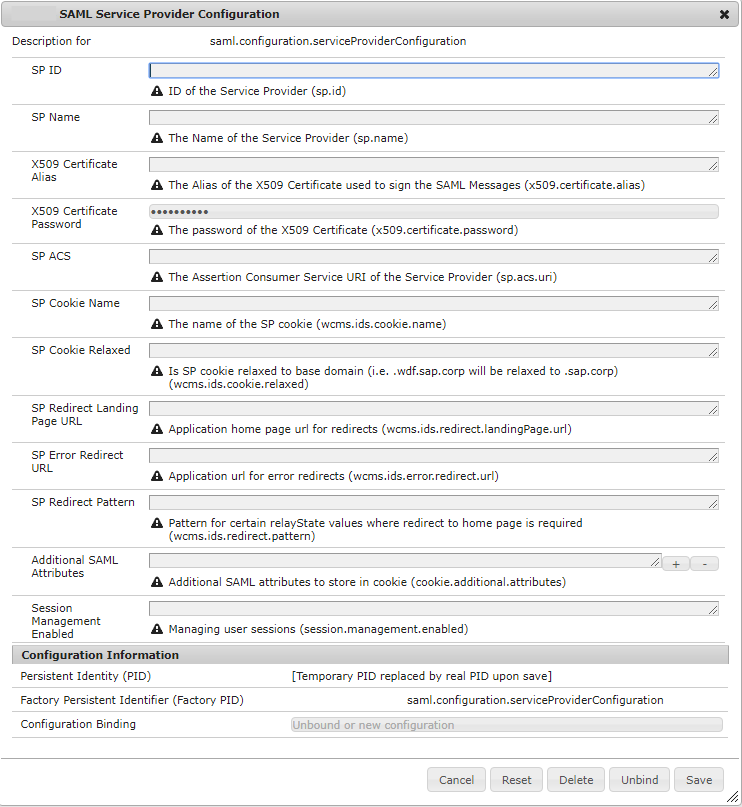
\includegraphics[width=\textwidth]{inc/svg/provider}
  \caption{Конфигурация поставщика сервиса}
  \label{fig:runConfig}
\end{figure}

\paragraph{Конфигурация поставщика учетных записей}

\begin{longlisting}
\inputminted[linenos,frame=single]{xml}{inc/src/samlConfiguration}
\caption{Конфигурация поставщика учетных записей} 
\label{lst:samlConfiguration}
\end{longlisting}

\begin{figure}[H]
  \centering
  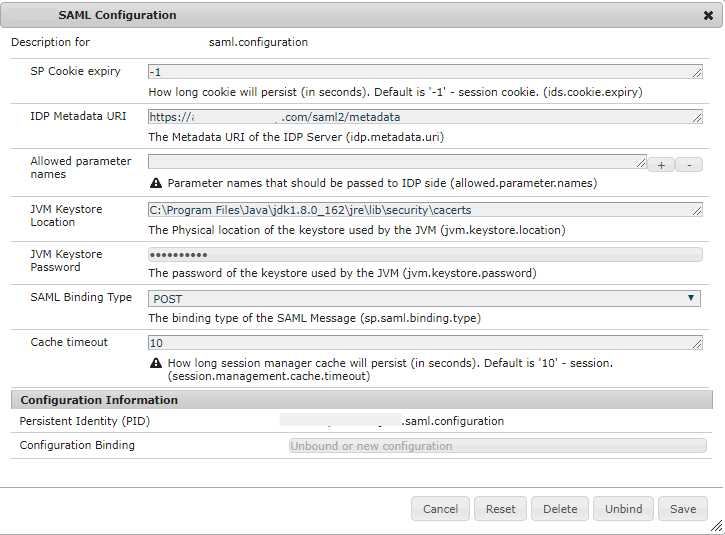
\includegraphics[width=\textwidth]{inc/svg/saml-config}
  \caption{Конфигурация поставщика учетных записей}
  \label{fig:samlConfig}
\end{figure}

\paragraph{Конфигурация авторизации на сайте}

\begin{longlisting}[H]
\inputminted[linenos,frame=single]{xml}{inc/src/idsConfiguration}
\caption{Код получения шифра} 
\label{lst:idsConfiguration}
\end{longlisting}

\begin{figure}[H]
  \centering
  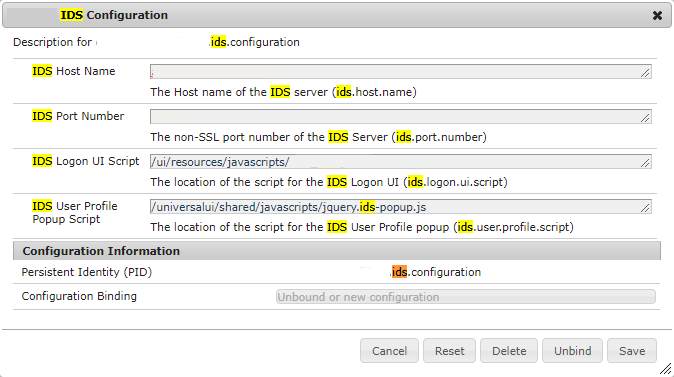
\includegraphics[width=\textwidth]{inc/svg/idsConfig}
  \caption{Конфигурация авторизации на сайте}
  \label{fig:idsConfig}
\end{figure}

%%% Local Variables:
%%% mode: latex
%%% TeX-master: "rpz"
%%% End:



%Не используемые на первой итерации, может потом удасться разбить проектирование на 2 раздела если потребуется, тогда будет использован ещё и impl.
%\chapter{Реализация}
\label{cha:impl}

\section{Разработка}
Разработку модуля необходимо начать с интеграции фреймворка Open SAML 3 с OSGI средой, затем будет рассмотрена разработка модулей авторизации и работы с SAML сообщениями.

\subsection{Интеграция Open SAML 3 со средой OSGI}
Как было выявлено в процессе выбора фреймворка, Open SAML 3 выполняет первоначальную инициализацию, загружая необходимые ресурсы и классы используя загрузчик классов не знающий о существование среды OSGI. Стандартный процесс инициализации фреймворка предполагает вызов метода initialize() сервиса org.opensaml.core.config.InitializationService. Данный сервис загружает все объекты которые необходимы для работы и регистрирует их в Java среде использую Java Services API с помощью сервиса org.opensaml.core.config.ConfigurationService. Для использования фреймворка в OSGI среде необходимо переопределить инициализацию фреймворка и поведение вышеописанных сервисов.

Для решения данной задачи было разработано три класса выполняющие первоначальную инициализацию фреймворка:
\begin{enumerate}
\item Activator - класс в котором заданы действия выполняющиеся при запуске модуля. В данном приложение метод активации извлекает загрузчик классов этого модуля и передает его в класс инициализации Open SAML 3, после чего вызывается метод SamlInitializationSupport.initialize(), листинг \ref{lst:activator}.
\item InitializationXMLConfigurator - класс наследует XMLConfigurator и подменяет загрузчик классов в методе createClassInstance(), листинг \ref{lst:xmlConfigurator}.
\item SamlInitializationSupport - основной класс инициализации, хранит все конфигурации и загрузчик классов модуля, приложение А листинг \ref{lst:samlInitialization}. Содержит следующие ключевые методы:
\begin{enumerate}
\item initializeXMLTooling - инициализирует все XML сервисы, перечисленные в списке конфигураций: configs[], использует переопределённый InitializationXMLConfigurator.
\item initializeAlgorithmRegistry -инициализирует алгоритмы используя загрузчик классов модуля.
\item initializeParserPool - инициализирует XML парсер.
\end{enumerate}
\end{enumerate}

\begin{longlisting}
\inputminted[linenos,frame=single]{java}{inc/src/Activator}
\caption{Метод активации модуля} 
\label{lst:activator}
\end{longlisting}

\begin{longlisting}
\inputminted[linenos,frame=single]{java}{inc/src/InitializationXMLConfigurator}
\caption{Класс инициализации XML конфигураций} 
\label{lst:xmlConfigurator}
\end{longlisting}

Данные классы выполняют инициализацию фреймворка Open SAML 3 во время активации модуля. Дальнейшая работа с фреймворком не требует специальных настроек и может выполняться как в классическом Java приложение.

\subsection{Подмодуль authentication}
Данный пакет предназначен для обработки запросов поступающих к сервису и является входной точкой приложения, диаграмма классов пакета представлена в приложение А рис.~\ref{fig:authenticationModule}. Пакет содержит следующие подпакеты и классы:
\begin{enumerate}
\item security.encryption
\item servlets
\item utils
\item Constatns
\item User
\item UserCookie
\end{enumerate}

\paragraph{Пакет security.encryption} содержит классы DesEncryptor и DesDecryptor  выполняющие шифрование и дешифрование значения куки с использованием алгоритма RSA/ECB/PKCS1Padding и стандартного Java класса javax.crypto.Cipher листинг \ref{lst:cipher}. Классы имеют методы decrypt() и encrypt() принимающие в качестве параметров строку которую необходимо зашифровать и ID поставщика сервиса. Ключ для шифрования извлекается из Java хранилища ключей, имя ключа извлекается из конфигурации модуля относящейся к переданному поставщику сервиса.

\begin{listing}[H]
\inputminted[linenos,frame=single]{java}{inc/src/cipher}
\caption{Код получения шифра} 
\label{lst:cipher}
\end{listing}

\paragraph{Пакет servlets} содержит сервлеты которые обрабатывают пользовательские запросы:
\begin{enumerate}
\item LoginServlet - Данный сервлет обрабатывает запросы на авторизацию либо ответы от поставщика учетных записей и имеет два сценария срабатывания:
\begin{enumerate}
\item Если поступил запрос на авторизацию от пользователя, то извлекается ID поставщика сервиса из селектора запроса с помощью которого будет получена конфигурация данного поставщика, затем составляется сообщение для поставщика учетных записей и выполняется его отправка.
\item Если в параметрах запроса обнаружен SAML ответ на авторизацию, то будет вызван обработчик AuthenticationResponseHandler.
\end{enumerate}
\item LogoutServlet -  Данный сервлет обрабатывает запросы на выход из системы либо ответы от поставщика учетных записей и имеет три сценария срабатывания:
\begin{enumerate}
\item Если в параметрах запроса обнаружен SAML ответ на запрос выхода из системы, то будет вызван обработчик LogoutResponseHandler. 
\item Если в параметрах запроса обнаружен SAML запрос на выход из системы, что означает запрос на выход из системы со стороны поставщика учетных записей, то будет вызван обработчик LogoutRequestHandler. 
\item Если поступил запрос на выход из системы от пользователя, получается конфигурация поставщика сервиса по аналогии с запросом авторизации, затем составляется и отправляется сообщение для поставщика учетных записей.
\end{enumerate}
\item UserInfo - Сервлет используемый для тестирования и влидации. Отображает информацию которая хранится о пользователи в куки.
\end{enumerate}

Данный пакет также содержит следующие обработчики запросов:
\begin{enumerate}
\item AuthenticationResponseHandler - обрабатывает и валидирует SAML ответы от поставщика учетных записей с помощью класса SamlAuthnResponseValidator. Если ответ прошел валидацию создается пользователь из полученных параметров SAML Assertion и сохраняются куки пользователя, пользователь перенаправляется на страницу для авторизованных пользователей либо на запрашиваемый ресурс.
\item LogoutRequestHandler - обрабатывает SAML запрос на выход из системы полученный от поставщика учетных записей. Удаляет куки пользователя, формирует и отправляет SAML сообщение для поставщика учетных записей о выполненной операции, после чего переправляет пользователя на страницу для не авторизованных пользователей.
\item LogoutResponseHandler - обрабатывает SAML ответ подтверждающий выход из системы полученный от поставщика учетных записей. Удаляет куки пользователя и переправляет его на страницу для не авторизованных пользователей.
\end{enumerate}

\paragraph{Пакет utils} содержит класс AuthUtils предназначенный для проверки передаваемых параметров на наличие XSS уязвимостей.

\paragraph{Класс Constatns} содержит константы путей по которым доступны сервлеты и значение куки которое должно быть задано при выходе из системы.
\paragraph{Класс User} представляет из себя модель пользователя и содержит все поля которые могут быть переданы поставщиком учетных записей вместе с ответом авторизации.
\paragraph{Класс UserCookie} представляет из себя модель куки пользователя и содержит набор значений которые хранятся в куки для пользователя:
\begin{enumerate}
\item userName - ID авторизованного пользователя.
\item sessionIndex - индекс сессии полученный от поставщика учетных записей.
\item user - объект пользователя полученный от поставщика учетных записей.
\end{enumerate}

\subsection{Подмодуль saml} 
Данный пакет предназначен для работы с SAML сообщениями а также конфигурации модуля, диаграмма классов пакета представлена в приложение А рис.~\ref{fig:samlModule}. Пакет содержит следующие подпакеты и классы:
\begin{enumerate}
\item bundle
\item configuration
\item messages
\item security
\item utils
\item validator
\end{enumerate}

\paragraph{Пакет bundle} содержит единственный класс Activator который был подробно рассмотрен в разделе "Интеграция Open SAML 3 со средой OSGI".
\paragraph{Пакет configuration} содержит сервисы конфигурации которые будут рассмотрены подробно в следующей секции данной главы.
\paragraph{Пакет messages} содержит классы осуществляющие генерацию SAML сообщений которые отправляются поставщику учетных записей и состоит из следующих классов:
\begin{enumerate}
\item BindingType - перечисляемый тип который содержит виды SAML привязки доступные в приложение. В текущей версии поддерживаются только POST и REDIRECT.
\item AbstractSamlMessage - абстрактный класс который содержит общие методы для всех SAML сообщений. Содержит следующие методы для работы с сообщениями:
\begin{enumerate}
\item generateUUID - генерирует ID которое служит идентификатором сообщения.
\item generateSigningParameters - генерирует параметры необходимые для подписи сообщения.
\item appendSigningData - подписывает сообщение в соответствие с типом привязки.
\item signObject - подписывает сообщение с помощью сертификата для типа привязки POST.
\item sendMessageToIDP - собирает сообщение и отправляет его поставщику учетных записей.
\end{enumerate}
\item SAML2AuthnRequestMessage - сообщение авторизации, код генерации сообщения в приложении А листинг \ref{lst:authMessage}.
\item SAML2LogoutRequestMessage - сообщение выхода из системы, код генерации сообщения в приложении А листинг \ref{lst:logoutMessage}.
\item SAML2LogoutResponseMessage - сообщение ответ на запрос выхода из системы со стороны поставщика учетных записей, код генерации сообщения в приложении А листинг \ref{lst:logoutResponseMessage}.
\end{enumerate}
\paragraph{Пакет security} содержит класс X509 который осуществляет взаимодействие с Java хранилищем ключей и предоставляет ключи для подписи сообщений или валидации полученных сообщений.
\paragraph{Пакет utils} содержит классы инициализации которые были рассмотрены ранее, а также вспомогательный класс SamlUtils со следующими методами:
\begin{enumerate}
\item getMessage - используется в обработчиках для извлечения SAML сообщения из запроса.
\item getMessageEncoder - используется в SAML сообщениях для задания сообщению кодировщика в соответствие с указанным в конфигурации типом  привязки.
\end{enumerate}
\paragraph{Пакет validator} содержит единственный класс SamlAuthnResponseValidator, который выполняет валидацию SAML ответа от поставщика учетных записей на запрос авторизации. Код валидации представлен в приложении А  листинг \ref{lst:validation}. В процессе валидации проверяется что структура сигнатуры верна и она подписана сертификатом который принадлежит поставщику учетных записей. Валидатор сигнатуры использует для работы Java Service API и требует отдельного переопределения для использования загрузчика классов модуля, листинг \ref{lst:activator}.

\begin{longlisting}
\inputminted[linenos,frame=single]{java}{inc/src/validatorLoader}
\caption{Код переопределения загрузчика классов валидатора} 
\label{lst:validatorLoader}
\end{longlisting}

\subsection{Конфигурация модуля}
Конфигурация модуля находится в пакете saml и содержит два вида конфигурации:
\begin{enumerate}
\item SamlConfigurationImpl - конфигурация которая содержит все элементы задающие используемый в системе поставщик учетных записей. Имеет следующие параметры:
\begin{enumerate}
\item idp.metadata.uri - URL метаданных IdP из которых извлекаются URL авторизации и выхода из системы.
\item jvm.keystore.location - путь до Java хранилища ключей в системе.
\item jvm.keystore.password - пароль Java хранилища ключей.
\item sp.saml.binding.type - тип SAML привязки, выбираемый параметр который может быть POST или REDIRECT.
\item ids.cookie.expiry - время жизни куки пользователя, если -1 время жизни приравнивается к времени жизни сессии.
\end{enumerate}
\item SamlServiceProviderConfigurationFactory - конфигурация которая задает параметры поставщика сервиса в системе. В системе может использоваться несколько различных поставщиков учетных записей с различными конфигурациями. Имеет следующие параметры:
\begin{enumerate}
\item sp.acs.uri - URL для обработки ответов от IdP и обработки утверждений.
\item sp.name - имя поставщика сервиса.
\item sp.id - идентификатор поставщика сервиса, используется для доступа к данной конфигурации.
\item x509.certificate.alias - имя сертификата который используется для подписи сообщений и валидации ответов от IdP.
\item x509.certificate.password - пароль от сертификата.
\item wcms.ids.cookie.name - имя под которым сохраняются куки пользователя.
\item wcms.ids.redirect.landingPage.url - URL на который переправляется пользователь после успешной авторизации.
\item wcms.ids.error.redirect.url - URL ошибок на который переправляется пользователь при возникновение ошибок в процессе авторизации.
\item wcms.ids.redirect.pattern - проверяет что URL перенаправления валдиный. 
\item cookie.additional.attributes - дополнительные параметры полученные от IdP.
\end{enumerate}
\item IdsConfigurationImpl - вспомогательная конфигурация, которая задает параметры позволяющие пользователю проходить авторизацию на стороне сайта или портала без перехода на сайт IdP. Имеет следующие параметры:
\begin{enumerate}
\item ids.host.name - адрес сервиса.
\item ids.port.number - порт сервиса.
\item ids.logon.ui.script - путь до скрипта пользовательского интерфейса.
\item ids.user.profile.script - путь до скрипта модального окна IdP.
\end{enumerate}
\end{enumerate}

\section{Тестирование}

Для оценки соответствия приложения заявленным требованиям было выполнено функциональное тестирование по тестовым сценариям. Тестирование проходило в два этапа, локально и на тестовом сервере компании. В тестирование принимало участие три независимых проекта использующих данный модуль и единый для всех поставщик учетных записей. Для проверки сценариев использовались бразуерные SAML плагины которые отображали SAML сообщения в запросах:

\begin{itemize}
\item SAML DevTools extension - для Chrome.
\item SAML-tracer - для Fire Fox.
\end{itemize}

\subsection{Тестирование сценария авторизации}
В таблице \ref{tab:testAuthn} приведены результаты тестирование сценария авторизации при котором использовалось два ресурса на которых выполнялся вход с настроенной конфигурацией используемого в компании поставщика учетных записей. Для обоих ресурсов использовался один и тот-же аккаунт.

\begin{longtable}{|p{5cm}|p{5cm}|l|}
  \caption{Результаты тестирования сценария авторизации}
  \label{tab:testAuthn}
  \\ \hline
  Шаг сценария & Ожидаемый результат & полученный результат  \\
  \hline \endfirsthead
  \subcaption{Продолжение таблицы~\ref{tab:testAuthn}}
  \\ \hline \endhead
  \hline \subcaption{Продолжение на след. стр.}
  \endfoot
  \hline \endlastfoot
  Пользователь отправляет запрос авторизации  
  & Приложение генерирует сообщение и перенаправляет пользователя на IdP вместе с этим сообщением
  & Соответствует \\
  \hline
  Пользователь проходит авторизацию на стороне IdP       			   
  & IdP перенаправляет пользователя обратно на сторону приложение вместе с SAML утверждением которое содержит данные пользователя и данные о созданной сессии
  & Соответствует \\
  \hline
  Приложение обрабатывает ответ               
  & Данные пользователя о сессии сохранены в куки и пользователю доступен контент
  & Соответствует \\
  \hline
\end{longtable}	

\subsection{Тестирование сценария выхода}
Для тестирования сценариев выхода из системы было использовано два портала использующих разработанный модуль.
\begin{itemize}
\item пользователь успешно авторизован на одном портале после чего инициализирует процесс выхода из системы (таблица \ref{tab:singleLogout}). 
\item пользователь авторизован на двух порталах и инициализирует процесс выхода из системы на одном из них (таблица \ref{tab:tripleLogout}).
\end{itemize}

\begin{longtable}{|p{5cm}|p{5cm}|l|}
  \caption{Результаты тестирования сценария выхода из системы для одного портала}
  \label{tab:singleLogout}
  \\ \hline
  Шаг сценария & Ожидаемый результат & полученный результат  \\
  \hline \endfirsthead
  \subcaption{Продолжение таблицы~\ref{tab:singleLogout}}
  \\ \hline \endhead
  \hline \subcaption{Продолжение на след. стр.}
  \endfoot
  \hline \endlastfoot
  Пользователь отправляет запрос выхода из системы  
  & Приложение генерирует сообщение и перенаправляет пользователя на IdP вместе с этим сообщением 
  & Соответствует \\
  \hline
  IdP удаляет сессию пользователя на своей стороне и посылает приложению сообщение об успешном выходе из системы       			   
  & Приложение получает ответ об успешном выходе из системы и очищает куки пользователя, после чего перенаправляет его на страницу авторизации
  & Соответствует \\
  \hline
\end{longtable}	

\begin{longtable}{|p{5cm}|p{5cm}|l|}
  \caption{Результаты тестирования сценария выхода из системы для нескольких порталов}
  \label{tab:tripleLogout}
  \\ \hline
  Шаг сценария & Ожидаемый результат & полученный результат  \\
  \hline \endfirsthead
  \subcaption{Продолжение таблицы~\ref{tab:tripleLogout}}
  \\ \hline \endhead
  \hline \subcaption{Продолжение на след. стр.}
  \endfoot
  \hline \endlastfoot
  Пользователь отправляет запрос выхода из системы  
  & Приложение генерирует сообщение и перенаправляет пользователя на IdP вместе с этим сообщением 
  & Соответствует \\
  \hline
  IdP находит все сессии, генерирует сообщения выхода для всех сервисов по очереди и перенаправляет пользователя на эти сервисы один за одним для осуществления выхода из системы.
  & Приложение получает запрос на выход из системы от IdP, очищает куки пользователя, генерирует ответ информирующий IdP об успешном выходе из системы и перенаправляет пользователя на IdP
  & Соответствует \\
  \hline
  IdP получает ответ о выходе из системы последнего сервиса, он генерирует сообщение ответ для приложения инициатора и перенаправляет пользователя в это приложение            
  & риложение получает ответ об успешном выходе из системы и очищает куки пользователя, после чего перенаправляет его на страницу авторизации
  & Соответствует \\
  \hline
\end{longtable}	


%\subsection{Блок-схема всякой ерунды}
%
%\subsubsection*{Кстати о заголовках}
%
%У нас есть и \Code{subsubsection}. Только лучше её не нумеровать.

\section{Конфигурация в системе}

Разработчики систем использующих данный модуль должны создать XML файлы конфигураций для всех настроек модуля. Примеры файлов для каждой конфигурации приведены ниже.

\paragraph{Конфигурация поставщика сервиса}

\begin{longlisting}
\inputminted[linenos,frame=single]{xml}{inc/src/samlProviderConfiguration}
\caption{онфигурация поставщика сервиса} 
\label{lst:samlProviderConfiguration}
\end{longlisting}

\begin{figure}[H]
  \centering
  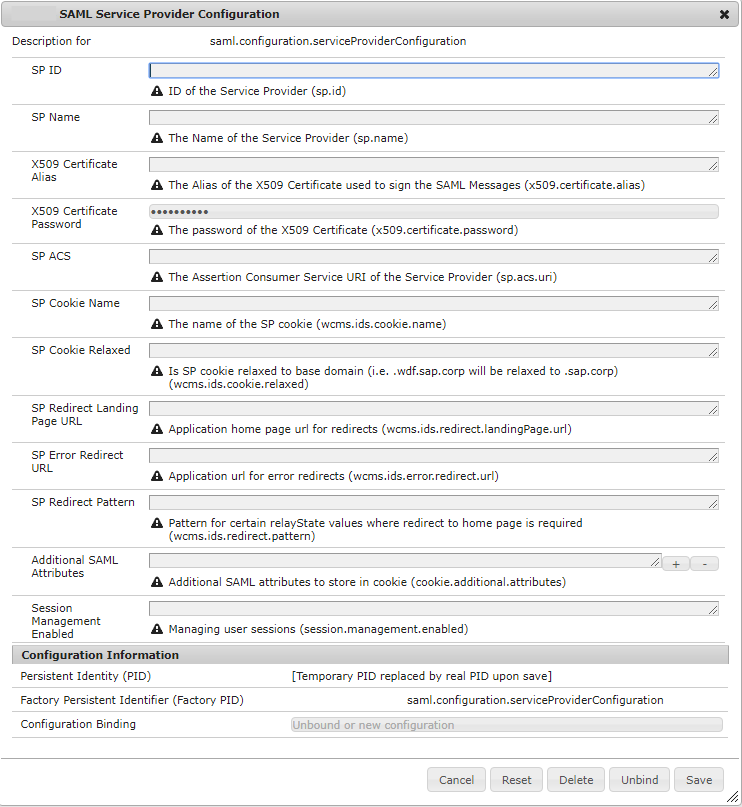
\includegraphics[width=\textwidth]{inc/svg/provider}
  \caption{Конфигурация поставщика сервиса}
  \label{fig:runConfig}
\end{figure}

\paragraph{Конфигурация поставщика учетных записей}

\begin{longlisting}
\inputminted[linenos,frame=single]{xml}{inc/src/samlConfiguration}
\caption{Конфигурация поставщика учетных записей} 
\label{lst:samlConfiguration}
\end{longlisting}

\begin{figure}[H]
  \centering
  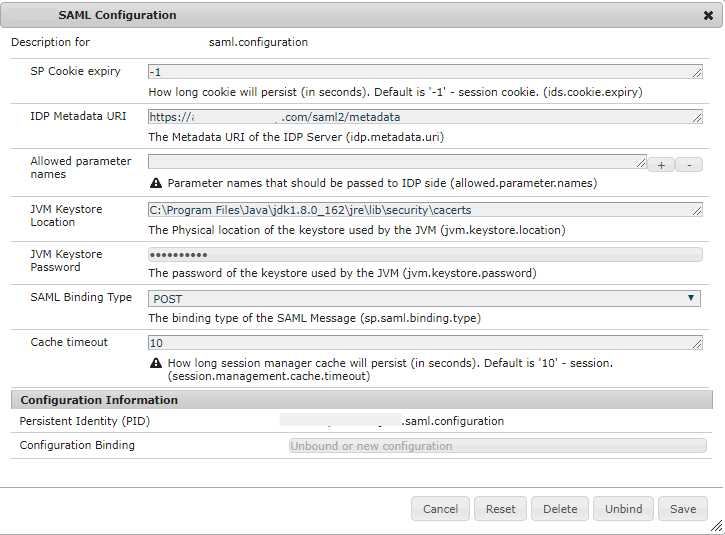
\includegraphics[width=\textwidth]{inc/svg/saml-config}
  \caption{Конфигурация поставщика учетных записей}
  \label{fig:samlConfig}
\end{figure}

\paragraph{Конфигурация авторизации на сайте}

\begin{longlisting}[H]
\inputminted[linenos,frame=single]{xml}{inc/src/idsConfiguration}
\caption{Код получения шифра} 
\label{lst:idsConfiguration}
\end{longlisting}

\begin{figure}[H]
  \centering
  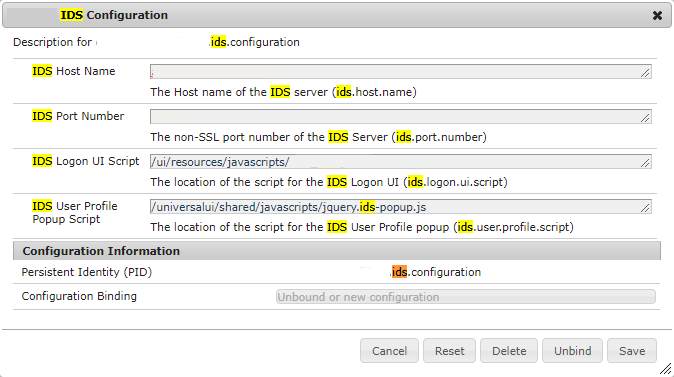
\includegraphics[width=\textwidth]{inc/svg/idsConfig}
  \caption{Конфигурация авторизации на сайте}
  \label{fig:idsConfig}
\end{figure}

%%% Local Variables:
%%% mode: latex
%%% TeX-master: "rpz"
%%% End:


%\include{50-research}
%\chapter{Организационно-экономический раздел}
\label{cha:econom}

%%% Local Variables:
%%% mode: latex
%%% TeX-master: "rpz"
%%% End:

%\chapter{Промышленная экология и безопасность}\label{cha:bzd}


%%% Local Variables:
%%% mode: latex
%%% TeX-master: "rpz"
%%% End:


\backmatter %% Здесь заканчивается нумерованная часть документа и начинаются ссылки и
            %% заключение

\Conclusion % заключение к отчёту

В ходе выполнения данной выпускной квалификационной работы были выполнены поставленные задачи.

В рамках работы были рассмотрены проблемы отслеживания состояния большого количества экземпляров системы AEM. Был проведен обзор системы и встроенных механизмов для отслеживания состояния. В результате анализа выявлены механизмы позволяющие дополнить систему требуемым функционалом.

На основе требований разработан пакет, и предложен способ интеграции с внешней программой мониторинга Nagios. Разработанный пакет имеет возможность дальнейшего расширения функционала в случае возникновения новых требований. Данный пакет успешно внедрен в системе заказчика.

%%% Local Variables: 
%%% mode: latex
%%% TeX-master: "rpz"
%%% End: 


% % Список литературы при помощи BibTeX
% Юзать так:
%
% pdflatex rpz
% bibtex rpz
% pdflatex rpz

\bibliographystyle{bibstyles/ugost2008}
\bibliography{rpz}

%%% Local Variables: 
%%% mode: latex
%%% TeX-master: "rpz"
%%% End: 


\appendix   % Тут идут приложения

\chapter{Диаграммы}
\label{cha:appendix1}

\begin{figure}
  \centering
  \includegraphics[scale=0.9]{inc/svg/complexDeploy}
  \caption{Схема развертывания AEM среды}
  \label{fig:complexDeploy}
\end{figure}

\begin{figure}
  \centering
  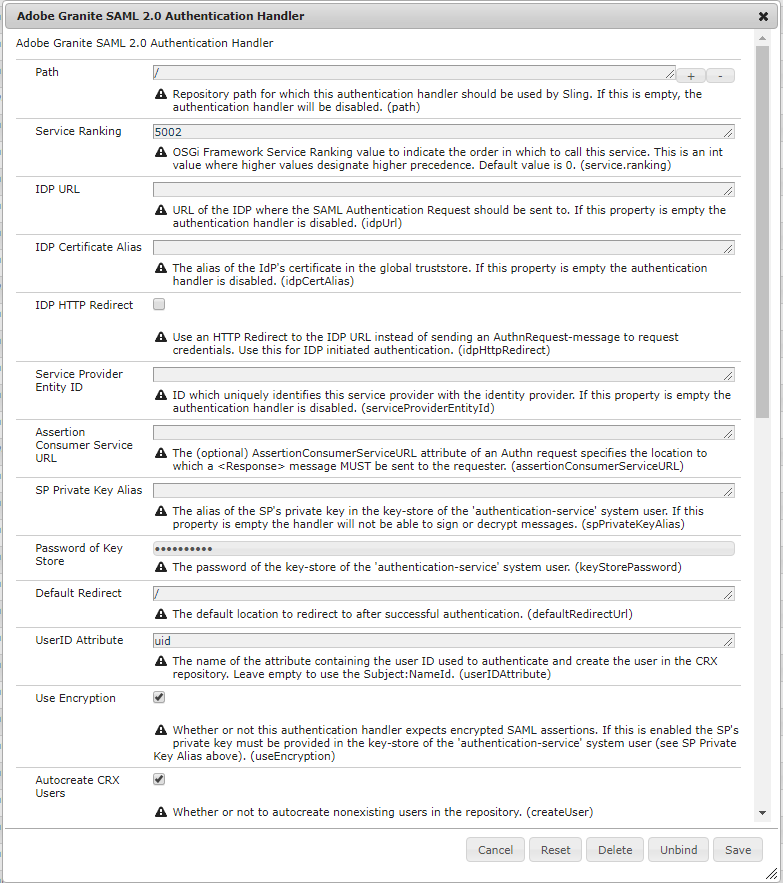
\includegraphics[width=\textwidth]{inc/img/handler1}
  \caption{Конфигурация 1 SAML 2.0 Authentication Handler}
  \label{fig:defaultHandlerConfig1}
\end{figure}

\begin{figure}
  \centering
  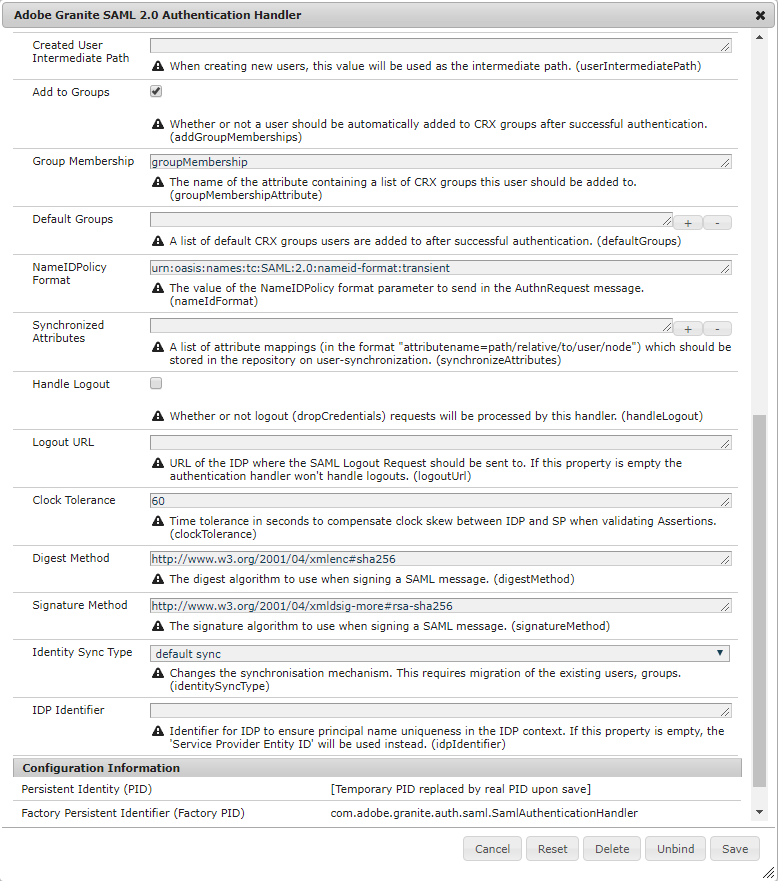
\includegraphics[width=\textwidth]{inc/img/handler2}
  \caption{Конфигурация 2 SAML 2.0 Authentication Handler}
  \label{fig:defaultHandlerConfig2}
\end{figure}

\begin{figure}
  \centering
  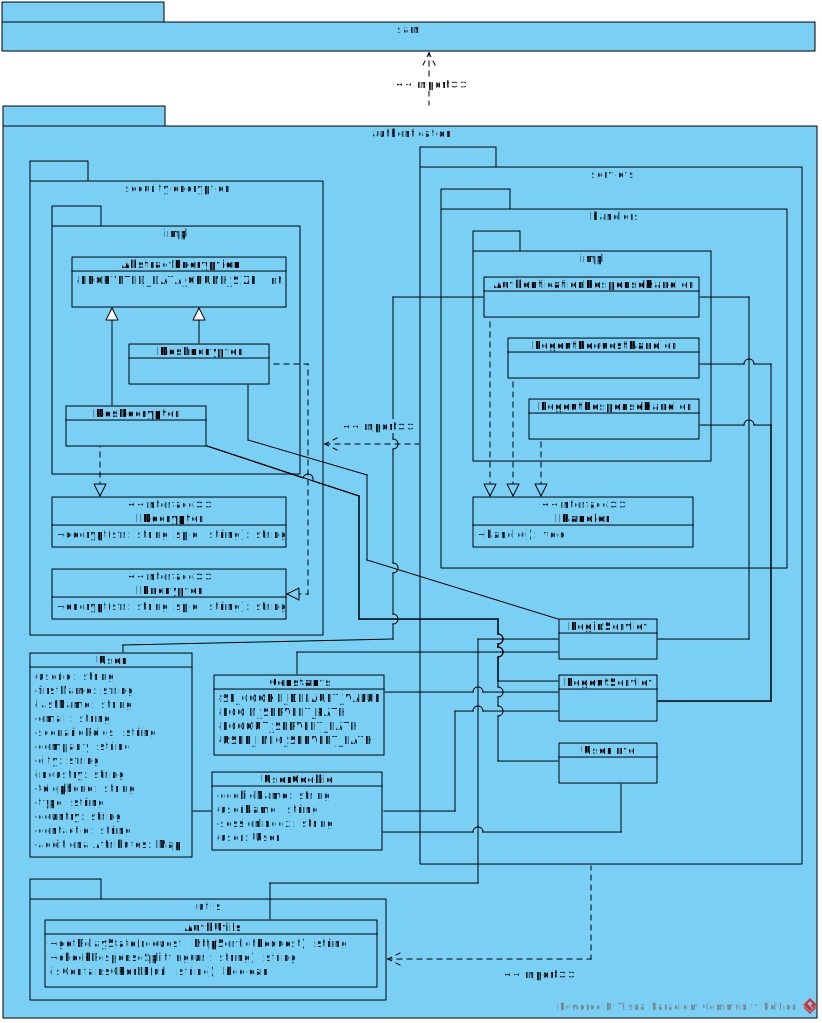
\includegraphics[width=\textwidth]{inc/svg/authenticationModule}
  \caption{Диаграмма классов пакета authentication}
  \label{fig:authenticationModule}
\end{figure}

\begin{figure}
  \centering
  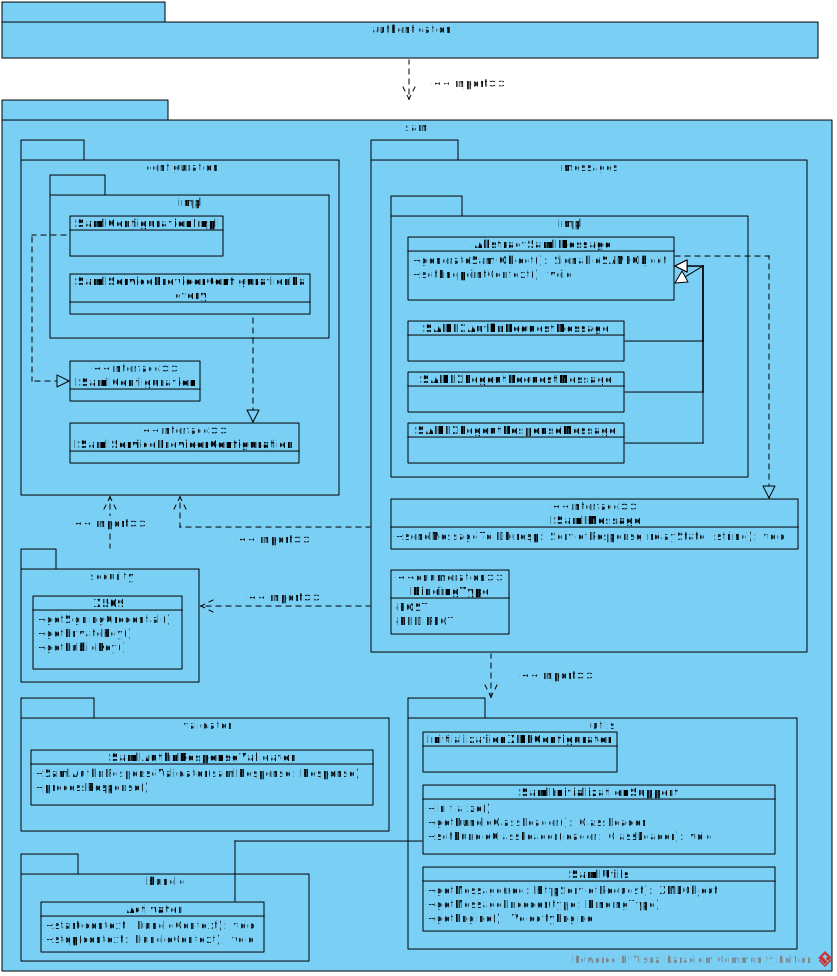
\includegraphics[width=\textwidth]{inc/svg/samlModule}
  \caption{Диаграмма классов пакета saml}
  \label{fig:samlModule}
\end{figure}

%%% Local Variables: 
%%% mode: latex
%%% TeX-master: "rpz"
%%% End: 

%\chapter{Еще картинки}
\label{cha:appendix2}

\begin{figure}
\centering
\caption{Еще одна картинка, ничем не лучше предыдущей. Но надо же как-то заполнить место.}
\end{figure}

%%% Local Variables: 
%%% mode: latex
%%% TeX-master: "rpz"
%%% End: 


\end{document}

%%% Local Variables:
%%% mode: latex
%%% TeX-master: t
%%% End:
